\documentclass[presentation]{beamer}
\usepackage{common}

\title[\lecturecode{07}]{07 \\ Addendum: patterns and recipes of functional programming}

\author[Mirko Viroli]{Mirko Viroli}
\institute[]{\texttt{mirko.viroli@unibo.it}}

\begin{document}

\frame[label=coverpage]{\titlepage}
\newcommand{\codepath}[1]{../../code/lecture-07/#1}

\section{FP and OOP}

\fr{Programming paradigms}{
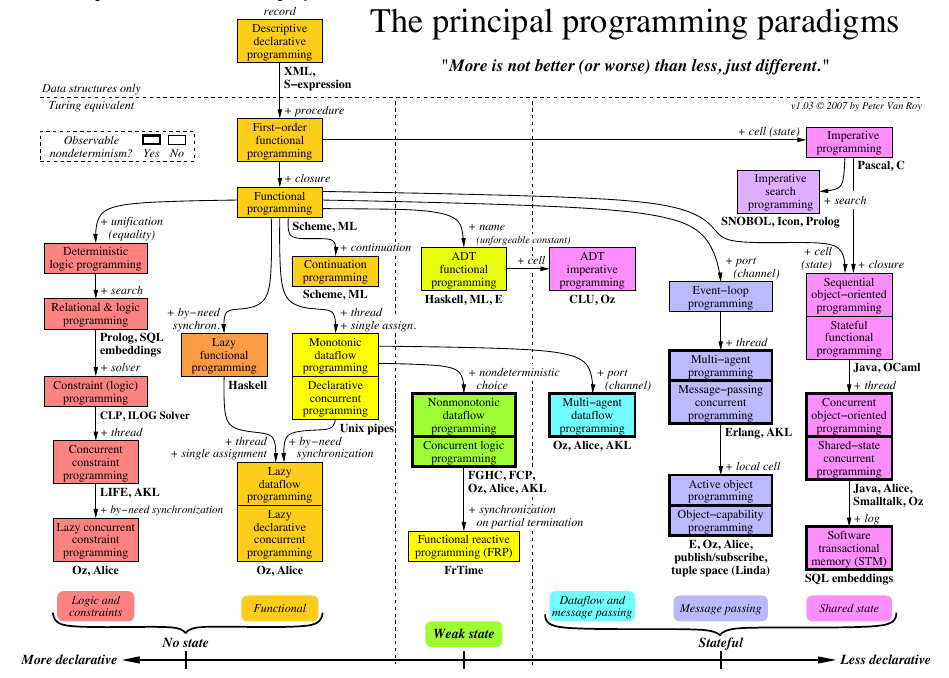
\includegraphics[height=0.9\textheight]{img/para.png}
}


\fr{Functional ideas outside functional languages}{
   \bl{Ideas of functional languages, recently brought e.g. in OO languages}{\iz{
    \item prefer immutability
    \item methods should better either change state or compute/return information
    \item methods should better be single expressions/statements
    \item separate construction logic from classes (see factory pattern)
    \item use of functions/lambdas as values (see strategy pattern)
    \item use of lazy-evaluation in data structures (see iterator)
    \item focus on ``what'' and not on ``how''
   }}
}


\section{Few recipes of functional programming}

\fr{Prefer immutability}{
    \codeview{1}{8}{40}{\tiny}{\codepath{PreferImmutability/Program.cs}}
}

\fr{Make defensive copies}{
    \codeview{1}{7}{38}{\tiny}{\codepath{DefensiveCopy/Program.cs}}
}


\fr{Consider static factories instead of constructors}{
  \codeview{1}{5}{36}{\tiny}{\codepath{PreferStaticFactories/Program.cs}}
}


\frs{5}{Hide implementations: only make available types}{
    \bl{The \cil{IOption<T>} case: a common functional block}{\iz{
        \item it represents information possibly not available
        \item note construction and hiding
    }}
    \codeview{1}{7}{30}{\tiny}{\codepath{NoExceptions/Program.cs}}
}

\fr{Don't abuse exceptions: use designed abstractions instead}{
    \codeview{1}{32}{52}{\tiny}{\codepath{NoExceptions/Program.cs}}
}


\end{document}

